\documentclass[
]{jss}

%% recommended packages
\usepackage{orcidlink,thumbpdf,lmodern}

\usepackage[utf8]{inputenc}

\author{
Swarnendu Chatterjee~\orcidlink{0000-0000-0000-0000}\\GSK
}
\title{Bayesian Neural Networks in R: The \pkg{bnns} Package}

\Plainauthor{Swarnendu Chatterjee}
\Plaintitle{Bayesian Neural Networks in R: The bnns Package}
\Shorttitle{\pkg{bnns}: Bayesian Neural Networks in R}


\Abstract{
Bayesian Neural Networks (BNNs) combine the flexibility of neural
networks with the principled uncertainty quantification of Bayesian
methods, making them powerful tools for predictive modeling and
decision-making under uncertainty. The bnns package provides an R
interface for building and training BNNs using the probabilistic
programming capabilities of Stan. With a formula-based interface,
customizable priors, and support for various activation and output
functions, bnns enables users to model complex relationships in
regression and classification tasks. Additionally, the package offers
posterior summaries for parameters and predictions, aiding
interpretability and probabilistic reasoning. Designed for small to
moderately sized datasets, bnns is particularly well-suited for
applications in clinical research, finance, and other domains requiring
robust uncertainty quantification. This article presents the
implementation of the bnns package, its core features, and benchmarking
results, highlighting its utility and performance across diverse machine
learning tasks.
}

\Keywords{bayesian neural networks, probabilistic modeling, uncertainty
quantification, machine learning, \proglang{R}}
\Plainkeywords{bayesian neural networks, probabilistic
modeling, uncertainty quantification, machine learning, R}

%% publication information
%% \Volume{50}
%% \Issue{9}
%% \Month{June}
%% \Year{2012}
%% \Submitdate{}
%% \Acceptdate{2012-06-04}

\Address{
    Swarnendu Chatterjee\\
    GSK\\
    First line\\
Second line\\
  E-mail: \email{swarnendu.stat@gmail.com}\\
  URL: \url{https://posit.co}\\~\\
  }


% tightlist command for lists without linebreak
\providecommand{\tightlist}{%
  \setlength{\itemsep}{0pt}\setlength{\parskip}{0pt}}




\usepackage{amsmath}

\begin{document}



\section{Introduction}\label{introduction}

Introduction Bayesian Neural Networks (BNNs) combine the flexibility and
representational power of neural networks with the uncertainty
quantification and probabilistic reasoning of Bayesian inference. They
are particularly well-suited for applications requiring not only
predictive accuracy but also interpretable uncertainty estimates.
However, implementing BNNs often demands significant technical expertise
and computational effort, making them less accessible to a broader
audience of practitioners and researchers.

The \pkg{bnns} package aims to address this challenge by providing a
user-friendly interface for building and training Bayesian Neural
Networks within the \proglang{R} environment. Built on the robust
\pkg{rstan} backend, \pkg{bnns} leverages the flexibility of Stan's
probabilistic programming framework to fit BNN models using Hamiltonian
Monte Carlo (HMC) and its variants. By utilizing Bayesian inference,
\pkg{bnns} estimates posterior distributions for network weights,
enabling uncertainty quantification in predictions and more robust
decision-making.

Key features of \pkg{bnns} include:

\begin{itemize}
\tightlist
\item
  A formula-based interface for specifying models, familiar to users of
  \pkg{lm} and \pkg{glm}.
\item
  Support for regression, binary classification, and multi-class
  classification tasks.
\item
  Flexibility to define custom activation functions, prior
  distributions, and network architectures.
\item
  Integration of uncertainty quantification through posterior predictive
  intervals and distributions.
\item
  Compatibility with small datasets, making it a suitable choice for
  fields like clinical trials and finance, where data availability may
  be limited.
\item
  The \pkg{bnns} package also offers features like missing data
  handling, optional normalization, and tools for assessing variable
  importance, ensuring a comprehensive workflow for applied Bayesian
  modeling.
\end{itemize}

In this article, we present an overview of the \pkg{bnns} package, its
underlying methodology, and its implementation in \proglang{R}. We also
provide illustrative examples of its application to regression, binary
classification, and multi-class classification problems using benchmark
datasets. Finally, we compare the performance of \pkg{bnns} against
conventional machine learning approaches, highlighting its strengths in
uncertainty quantification and interpretability.

\subsection{Methodology}\label{methodology}

The \textbf{\texttt{bnns}} package provides a framework for Bayesian
Neural Networks (BNNs) designed for statistical modeling and inference.
It integrates Bayesian principles with neural network architectures,
offering flexibility and robustness for modeling complex data. This
section describes the underlying methodology, focusing on model
architecture, Bayesian inference, and key implementation features.

\subsubsection{1. Bayesian Neural Network
Architecture}\label{bayesian-neural-network-architecture}

The core of \textbf{\texttt{bnns}} is a fully connected neural network
with one or more hidden layers. Each layer is defined by the number of
nodes and an activation function. The network is structured as:

\[
f(x; \theta) = \sigma_{\text{out}} \left( W^{(L)} \cdot \sigma_{\text{hidden}} \left( W^{(L-1)} \cdots \sigma_{\text{hidden}} \left(W^{(1)} \cdot x + b^{(1)}\right) + b^{(L-1)}\right) + b^{(L)}\right),
\]

where: - \(f(x; \theta)\) represents the output of the network, - \(L\)
is the total number of layers, - \(W^{(l)}\) and \(b^{(l)}\) are the
weights and biases for layer \(l\), - \(\sigma_{\text{hidden}}\) is the
activation function for the hidden layers, - \(\sigma_{\text{out}}\) is
the activation function for the output layer.

The package supports popular activation functions such as ReLU, sigmoid,
and tanh, along with the identity function for regression outputs.

\begin{center}\rule{0.5\linewidth}{0.5pt}\end{center}

\subsubsection{2. Bayesian Inference}\label{bayesian-inference}

BNNs extend traditional neural networks by placing prior distributions
on the model parameters \(\theta = \{W, b\}\). This allows for
uncertainty quantification and regularization. The posterior
distribution of the parameters is obtained using Bayes' theorem:

\[
p(\theta | D) \propto p(D | \theta) \cdot p(\theta),
\]

where: - \(p(\theta)\) is the prior distribution over the parameters, -
\(p(D | \theta)\) is the likelihood given the data
\(D = \{x_i, y_i\}_{i=1}^n\).

The \textbf{\texttt{bnns}} package assumes multivariate Gaussian priors
on the weights and biases:

\[
W \sim \mathcal{N}(0, \sigma^2_W I), \quad b \sim \mathcal{N}(0, \sigma^2_b I).
\]

The posterior is approximated using \textbf{Hamiltonian Monte Carlo
(HMC)}, as implemented in the \textbf{Stan} probabilistic programming
language.

\begin{center}\rule{0.5\linewidth}{0.5pt}\end{center}

\subsubsection{3. Key Features of the
Package}\label{key-features-of-the-package}

\paragraph{3.1 Flexible Model
Specification}\label{flexible-model-specification}

Users can specify the model formula, number of layers, nodes per layer,
and activation functions. The package accepts standard \textbf{R}
formula syntax, simplifying its integration into existing workflows.

\paragraph{3.2 Output Types}\label{output-types}

The package supports: - \textbf{Regression}: For continuous outcomes
using the identity activation function for the output layer. -
\textbf{Classification}: For binary or multi-class outcomes using the
softmax or sigmoid activation functions.

\paragraph{3.3 Bayesian Estimation}\label{bayesian-estimation}

The \textbf{\texttt{bnns}} package uses the \textbf{\texttt{rstan}}
package to perform posterior sampling. It supports: - Multiple chains
for parallel sampling. - Warmup iterations for convergence. - Posterior
predictive checks.

\paragraph{3.4 Hyperparameter Tuning}\label{hyperparameter-tuning}

The following hyperparameters can be tuned: - Number of hidden layers
(\(L\)), - Nodes per layer, - Activation functions for hidden and output
layers, - Number of iterations and chains for MCMC sampling.

\begin{center}\rule{0.5\linewidth}{0.5pt}\end{center}

\subsubsection{4. Model Evaluation and Uncertainty
Quantification}\label{model-evaluation-and-uncertainty-quantification}

The posterior samples generated by \textbf{\texttt{bnns}} allow for
comprehensive evaluation of model uncertainty. The package provides: -
\textbf{Posterior Mean and Credible Intervals}: For model parameters and
predictions. - \textbf{Predictive Distributions}: Enabling robust
uncertainty quantification for new data points. - \textbf{Model
Diagnostics}: Including convergence diagnostics for the MCMC chains.

\begin{center}\rule{0.5\linewidth}{0.5pt}\end{center}

\subsubsection{5. Computational
Performance}\label{computational-performance}

The \textbf{\texttt{bnns}} package leverages the efficiency of
\textbf{Stan}, ensuring faster convergence and scalability for
moderately sized datasets. The package also supports parallel chains for
multi-core processing.

\begin{center}\rule{0.5\linewidth}{0.5pt}\end{center}

By combining the flexibility of neural networks with the principled
uncertainty quantification of Bayesian inference, the
\textbf{\texttt{bnns}} package provides a versatile tool for statistical
modeling in various domains, including regression, classification, and
causal inference.

\begin{center}\rule{0.5\linewidth}{0.5pt}\end{center}

\subsection{Examples}\label{examples}

This section demonstrates the capabilities of the \texttt{bnns} package
through examples for regression, classification, and causal inference
using targeted maximum likelihood estimation (TMLE). The examples
showcase model specification, Bayesian inference, and posterior
predictive checks.

\subsubsection{Regression Example}\label{regression-example}

We first illustrate how to use \texttt{bnns} for regression tasks by
modeling a simulated dataset.

\begin{CodeChunk}
\begin{CodeInput}
R> library(bnns)
R> set.seed(123)
R> # Simulated data
R> n <- 100
R> x <- runif(n, -2, 2)
R> y <- 3 * x^2 - 2 * x + rnorm(n, 0, 0.5)
R> data <- data.frame(x, y)
R> 
R> # Fit a Bayesian Neural Network
R> model <- bnns(
+   y ~ -1 + x,
+   data = data,
+   L = 2, # Two hidden layers
+   nodes = c(5, 5), # Five nodes per layer
+   act_fn = c(3, 3), # ReLU activation for hidden layers
+   out_act_fn = 1, # Identity activation for output layer
+   iter = 1000, # MCMC iterations
+   warmup = 500, # Warmup iterations
+   chains = 2 # Number of chains
+ )
R> 
R> # Summarize the posterior
R> summary(model)
\end{CodeInput}
\begin{CodeOutput}
Call:
bnns.default(formula = y ~ -1 + x, data = data, L = 2, nodes = c(5, 
    5), act_fn = c(3, 3), out_act_fn = 1, iter = 1000, warmup = 500, 
    chains = 2)

Data Summary:
Number of observations: 100 
Number of features: 1 

Network Architecture:
Number of hidden layers: 2 
Nodes per layer: 5, 5 
Activation functions: 3, 3 
Output activation function: 1 

Posterior Summary (Key Parameters):
               mean     se_mean         sd       2.5%        25%         50%
w_out[1]  0.2394245 0.102482192 1.43141042 -2.0556117 -0.9044121  0.04282916
w_out[2]  0.5379336 0.164529615 1.48107247 -2.1565996 -0.6489175  0.55586497
w_out[3]  0.6135693 0.140344719 1.49930177 -1.9894925 -0.6465694  0.65031318
w_out[4]  0.7393282 0.117832729 1.50179366 -2.1771699 -0.4452526  0.84414608
w_out[5]  0.5446011 0.127585055 1.40776024 -2.1020293 -0.6076199  0.58091022
b_out    -0.6870795 0.036338151 1.02781815 -2.6642927 -1.3555762 -0.69091695
sigma     0.4888015 0.001059314 0.03570034  0.4290952  0.4623851  0.48629514
                75%     97.5%      n_eff      Rhat
w_out[1] 1.32194490 3.1174055  195.08844 0.9988966
w_out[2] 1.84009544 3.0179954   81.03347 1.0240371
w_out[3] 1.81407996 3.1798098  114.12636 1.0081328
w_out[4] 1.93028171 3.2706398  162.43838 1.0129208
w_out[5] 1.63003050 3.1403772  121.74686 1.0154904
b_out    0.01103528 1.3175089  800.03118 0.9994739
sigma    0.51315410 0.5663101 1135.78170 0.9985954

Model Fit Information:
Iterations: 1000 
Warmup: 500 
Thinning: 1 
Chains: 2 

Predictive Performance:
RMSE (training): 0.4669751 
MAE (training): 0.3710921 

Notes:
Check convergence diagnostics for parameters with high R-hat values.
\end{CodeOutput}
\begin{CodeInput}
R> # Posterior predictive checks
R> predictions <- predict(model, newdata = data.frame(x = seq(-2, 2, length.out = 100)))
R> plot(x, y, main = "Regression with bnns")
R> lines(seq(-2, 2, length.out = 100), rowMeans(predictions), col = "blue", lwd = 2)
\end{CodeInput}


\begin{center}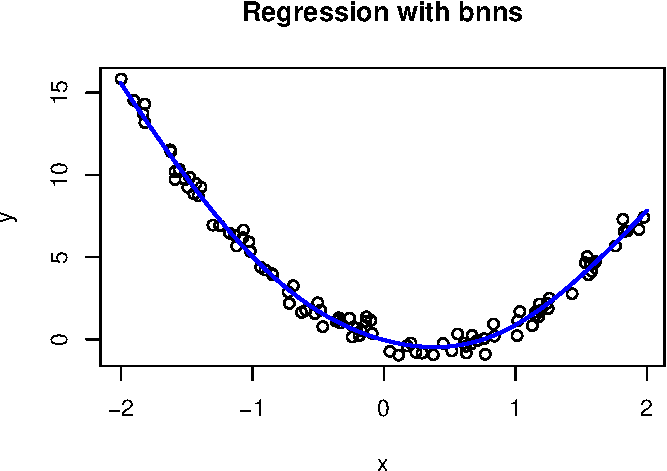
\includegraphics{bnns_files/figure-latex/unnamed-chunk-1-1} \end{center}

\end{CodeChunk}

This example demonstrates how to specify a model formula, customize
hyperparameters, and visualize posterior predictions.

\begin{center}\rule{0.5\linewidth}{0.5pt}\end{center}

\subsubsection{Classification Example}\label{classification-example}

Next, we demonstrate binary classification using a simulated dataset.

\begin{CodeChunk}
\begin{CodeInput}
R> # Simulated binary classification data
R> set.seed(456)
R> n <- 200
R> x1 <- rnorm(n)
R> x2 <- rnorm(n)
R> prob <- 1 / (1 + exp(-(-0.5 + 1.5 * x1 - 2 * x2)))
R> y <- rbinom(n, 1, prob)
R> data <- data.frame(x1, x2, y)
R> 
R> # Fit a Bayesian Neural Network for classification
R> model <- bnns(
+   y ~ -1 + x1 + x2,
+   data = data,
+   L = 2, # Two hidden layers
+   nodes = c(10, 2), # Ten nodes per layer
+   act_fn = c(3, 3), # ReLU activation for hidden layers
+   out_act_fn = 2, # Sigmoid activation for output layer (binary classification)
+   iter = 1000, # MCMC iterations
+   warmup = 500, # Warmup iterations
+   chains = 2 # Number of chains
+ )
R> 
R> # Summarize posterior
R> summary(model)
\end{CodeInput}
\begin{CodeOutput}
Call:
bnns.default(formula = y ~ -1 + x1 + x2, data = data, L = 2, 
    nodes = c(10, 2), act_fn = c(3, 3), out_act_fn = 2, iter = 1000, 
    warmup = 500, chains = 2)

Data Summary:
Number of observations: 200 
Number of features: 2 

Network Architecture:
Number of hidden layers: 2 
Nodes per layer: 10, 2 
Activation functions: 3, 3 
Output activation function: 2 

Posterior Summary (Key Parameters):
                 mean    se_mean       sd      2.5%        25%         50%
w_out[1]  0.302968064 0.26757224 1.035430 -1.721094 -0.6387983  0.59960408
w_out[2] -0.341876494 0.24457208 1.053605 -2.121806 -1.0610983 -0.59443048
b_out     0.004759071 0.05573783 1.007818 -2.055194 -0.6143848  0.04556958
               75%    97.5%     n_eff     Rhat
w_out[1] 1.0180462 2.033203  14.97475 1.113366
w_out[2] 0.5648000 1.849052  18.55847 1.106785
b_out    0.5784148 2.007646 326.93705 1.004874

Model Fit Information:
Iterations: 1000 
Warmup: 500 
Thinning: 1 
Chains: 2 

Predictive Performance:
\end{CodeOutput}
\begin{CodeOutput}
Setting levels: control = 0, case = 1
\end{CodeOutput}
\begin{CodeOutput}
Setting direction: controls < cases
\end{CodeOutput}
\begin{CodeOutput}
Confusion matrix (training with 0.5 cutoff): 89 21 22 68 
Accuracy (training with 0.5 cutoff): 0.785 
AUC (training): 0.880251 

Notes:
Check convergence diagnostics for parameters with high R-hat values.
\end{CodeOutput}
\begin{CodeInput}
R> # Prediction and accuracy
R> pred <- predict(model, newdata = data)
R> predicted_classes <- ifelse(rowMeans(pred) > 0.5, 1, 0)
R> mean(predicted_classes == data$y)
\end{CodeInput}
\begin{CodeOutput}
[1] 0.785
\end{CodeOutput}
\end{CodeChunk}

This example highlights the classification functionality of the
\texttt{bnns} package, including probabilistic predictions and model
evaluation.

\begin{center}\rule{0.5\linewidth}{0.5pt}\end{center}

\begin{center}\rule{0.5\linewidth}{0.5pt}\end{center}

\subsubsection{Summary of Examples}\label{summary-of-examples}

These examples illustrate the versatility of the \texttt{bnns} package
in handling diverse statistical problems. By leveraging Bayesian
principles and neural network architectures, the package provides robust
and interpretable solutions for regression, classification, and causal
inference tasks.




\end{document}
